% Chapter Template

\chapter{Theoretical overview} % Main chapter title

\label{Chapter2} % Change X to a consecutive number; for referencing this chapter elsewhere, use \ref{ChapterX}

\lhead{Chapter 2. \emph{Theoretical overview}} % Change X to a consecutive number; this is for the header on each page - perhaps a shortened title

Standard model of elementary particles is a theory emerged in 1960s and 1970s describing all of the known elementary particles and interactions except gravity. The final formulation of Standard model incorporates several theories: quantum electrodynamics, Glashow-Weinberg-Salam theory of electroweak processes and quantum chromodynamics, all of them describing the relations between quarks and fermions. There evidences which show the Standard model is not a final theory of elementary particles, but so far it's predictions were confirmed every time through numerous experimental tests. Standard model has one additional nice property, all fundamental interactions arise from one general principle, the requirement of local gauge invariance. \\
In this chapter a brief overview of the standard model particles and interactions will be shown with the emphasis on the W boson and b quarks which are the most relevant for this thesis. Cross section detremination at hadron colliders will be shown.  In the last part of the chapter historical account of the development of W+b-jets theoretical calculations is described together with the existing experimental results.

%----------------------------------------------------------------------------------------
%	SECTION 1
%----------------------------------------------------------------------------------------

\section{Standard model overview}



 



%-----------------------------------
%	SUBSECTION 1.2
%-----------------------------------
\subsection{Elementary particles of Standard model}

\subsubsection{b quarks}

\subsubsection{Discovery and role of W boson}


%-----------------------------------
%	SUBSECTION 1.2
%-----------------------------------
\subsection{Electroweak interactions}

%Konačni cilj ovog kratkog teorijskog razmatranja je pokazati elektroslabo ujedinjenje i procijeniti mase baždarnih bozona. Prvi korak na tom putu je naći lagranžijan invarijantan na SU$(2)_L\times$U$(1)_Y$ transformacije. Budući da su elementarne čestice fermioni spina $\frac{1}{2}$, njih opisuje Diracov Lagrangian:
%
%\begin{equation}
%\mathcal{L}= \overline{\psi}(i\gamma^{\mu}\partial_{\mu}-m)\psi
%\label{eq:Dirac_lagr}
%\end{equation} 
%
%Ovaj lagranžijan je invarijantan na globalnu U(1) transformaciju, medutim na taj se lagranžijan postavlja dodatni zahtjev lokalne baždarne invarijantnosti, tj. želi se neovisnost fizikalnih faza o tome koja se faza odnosno baždarenje odabere. Takva transformacija poprima oblik:
%
%\begin{equation}
%U=e^{-iq\alpha(x)}
%\label{eq:u1}
%\end{equation}
%
%Uvrštavanjem takve transformacije u (\ref{lagrangijan}) vidljivo je da zbog $\partial_{\mu} \alpha(x) \neq 0$ lagranžijan nije invarijantan. Medutim, lagranžijan može postati invarijantan ako uvedemo baždarno polje $B_{\mu} (x)$ koje se transformira kao:
%
%\begin{equation}
%B_\mu\rightarrow B_{\mu}'=B_{\mu}+\partial_\mu \alpha(x)
%\label{eq:be}
%\end{equation} 
%
%Nadalje, $B_\mu$ se koristi kako bi se derivacija pretvorila u kovarijantnu derivaciju:
%\begin{equation}
%D_\mu=\partial_{\mu} +iqB_\mu 
%\label{eq:kovdev}
%\end{equation}
%
%Sada transformacija postaje:
%
%\begin{equation}
%D_\mu \psi\rightarrow D_\mu \psi' = e^{-iq\alpha(x)} D_\mu \psi 
%\label{eq:trans}
%\end{equation} 
%
%Lagranžijan mora sadržavati i kinetički član, tako da on sada glasi:
%
%\begin{equation}
%\mathcal{L}=\overline{\psi}(\gamma^{\mu} D_{\mu}+m)\psi + \frac{1}{4}F^{\mu \nu} F_{\mu \nu}
%\label{eq:u1lagr}
%\end{equation}
%
%gdje je $F_{\mu \nu}= \partial^{\mu} B^{\nu} + \partial^{\nu} B^{\mu}$ tenzor energije i momente koji je invarijantan na transformacije (\ref{be}). Lagranžijan, kada se raspiše, sadrži član $g\overline{\psi}\gamma_\mu\psi B_{\mu}$ koji opisuje vezanje fotona. Važnost ovog lagranžijana je u tome što ne dopušta fotonski maseni član $m_{\gamma}^2 B_{\mu}B^{\mu}$ budući da takav član naručava lokalnu baždarnu invarijantnost.\\
%
%SU(2) simetriju uvodimo u standardni model jednako kao i U(1) simetriju, ali uzimajući u obzir njezinu bogatiju grupnu strukturu. Teorija grupa kaže da simetrija SU(2) ima $2^2-1=3$ generatora transformacije, za razliku od $U(1)$ transformacije koja ima samo jedan generator. Ova grupa je neabelova što se odražava u činjenici da njeni generatori ne komutiraju, stoga algebra ove grupe glasi:
%\begin{equation}
%[T_i,T_j]=\epsilon _{ijk} T_k
%\label{eq:comutator}
%\end{equation}
%Generatori $T_i$ generiraju specijalne unitarne lokalne transformacije oblika $U(\theta)=e^{-ig_w \mathbf{T}.\mathbf{\theta(x)}}$ gdje je $g_w$ konstanta vezanja. $T_i$ su povezani s baždarnim poljima $W_{\mu}^{i}$ koja se pod SU(2) transformiraju kao:
%\begin{equation}
%\mathbf{T.W'_{\mu}}=U(\theta)\mathbf{T.W_{\mu}}U^{-1}(\theta)+ \frac{i}{g}(\partial _{\mu}U(\theta))U^{-1}(\theta)
%\label{eq:transform}
%\end{equation}
%Zbog očuvanja lokalne baždarne invarijantnosti, opet običnu derivaciju moramo zamijeniti kovarijantnom:
%\begin{equation}
%D_{\mu}=\partial_{\mu}+ig\mathbf{T.W_{\mu}}
%\label{eq:kovarder}
%\end{equation}
%čija su svojstva analogna onima U(1) transformacije:
%
%\begin{equation}
%D_{\mu} \psi^{t} \rightarrow D_{\mu} \psi^{t'} = U(\theta) D_{\mu} \psi^{t} 
%\label{eq:trans}
%\end{equation} 
%gdje je $\psi^{(t)}$ SU(2) multiplet. Kovarijantna derivacija povezuje interakcije SU(2) baždarnih polja i čestica prikazanih sa $\psi^{(t)}$. Potrebno je uvesti i član:
%\begin{equation}
%\mathbf{F}^{\mu \nu}=\partial^{\mu} \mathbf{W}^{\nu}- \partial^{\nu} \mathbf{W}^{\mu}-g\mathbf{W}^{\mu}\times\mathbf{W}^{\nu}
%\label{eq:ef}
%\end{equation} 
% Ovaj izraz se razlikuje od izraza za U(1) grupu u zadnjem članu $g\mathbf{W}^{\mu}\times\mathbf{W}^{\nu}$ gdje do izražaja dolazi neabelovska priroda grupe SU(2). Konstanta vezanja $g$ upućuje na postojanje naboja koje prenosi baždarno polje. Konačni SU(2) langranžijan glasi:
% \begin{equation}
%\mathcal{L}=\overline{\psi}^{(t)}(\gamma^{\mu} D_{\mu}+m)\psi^{(t)} + \frac{1}{4}\mathbf{F}^{\mu \nu} \mathbf{F}_{\mu \nu}
%\label{eq:su2lagr}
%\end{equation}
%
%Maseni član za baždarne bozone SU(2) simetrije bi narušio baždarnu invarijantnost teorije. Budući da je poznato da ti bozoni imaju masu, uveden je Glashow-Salam-Weinbergov model koji kaže da je simetrija elektroslabe teorije SU(2)$_L\times$U(1)$_Y$. Naboji, tj. generatori takve simetrije su elektroslabi izospin $t$ i elektroslabi hipernaboj $Y$. 
%Slabi hipernaboj se računa kao:
%\begin{equation}
% Y=2(Q-t_3)
%\label{eq:hyprecharge}
%\end{equation}
%gdje je $Q$ naboj čestice, a $t_3$ je projekcija izospina. 
%Eksperimentalno je opaženo da se baždarna polja vežu samo na lijeve fermione, koji se mogu svrstati u SU(2) dublete $$L=\left(\begin{array}{c}\nu_{e}\\ e\end{array} \right)_{L}$$ te im se pridjeljuju odgovarajući kvantni brojevi izospina. Takvi dubleti čine lijevu komponentu Diracovih spinora, što znači da ukupne spinore možemo rastaviti na lijeve i desne:
%\begin{align}
% \psi_L&=P_L \psi= \frac{1- \gamma_5}{2}\psi \\
% \psi_R&=P_R \psi= \frac{1+ \gamma_5}{2}\psi \\
%\end{align}
%
%Iz takve podjele fermiona vidljiva su neka svojstva slabih interakcija. Razlika naboja unutar jednog dubleta je uvijek jednaka jedan, što znači da baždarna polja odgovorna za njihov medusobni prijelaz mora imati naboj $\pm 1$. Prijelazi medu leptonima su ograničeni na jednu generaciju, tj. nema medugeneracijskih prijelaza, što se očituje očuvanjem leptonskog broja. 
%
%Podjela na lijeve i desne fermione na SU(2) multiplete i uvrštavanje njihovog masenog člana u lagranžijan bi slomilo simetriju buduću da $m \psi \overline{\psi}$ veže lijeve i desne komponente spinora. Ako SU(2) transformacije imaju utjecaja samu na lijeve spinore, taka je baždarna invarijantnost narušena. Mase fermiona ulaze u teoriju preku Higgsovog mehanizma o kojem će više riječi biti u idućem odjeljku.
%                                                                                                     
%Kombinirana $SU(2)_L \times U(1)_Y$ teorija daje 4 baždarna bozona koja su i opažena u prirodi. Lagranžijan ovih baždarnih bozona dan je izrazom \ref{equ:bazdarnilangrangian}.
%\begin{equation}
% L_G=\frac{1}{4} F_{\mu\nu}F^{\mu\nu} + \frac{1}{4}B_{\mu\nu}B^{\mu}
%\end{equation}
%gdje je $F_{\mu\nu}$ tenzor energije i impulsa za baždarne bozone $SU(2)$ grupe, dok se $B_{\mu\nu}$ odnosi na U(1) baždarne bozone. Ovi su bozoni bezmaseni, što znači da ne opisuju stvarna fizikalna stanja. Takvo ponašanje upućuje na činjenicu da je simetrija $SU(2)_L \times U(1)_Y$ slomljena te se uvodi Higgsov mehanizam.

%-----------------------------------
%	SUBSECTION 1.3
%-----------------------------------

\subsection{Higgs mechanism}


%Uvjet ekstremizacije neke energetske veličine može dovesti do loma simetrije sustava. Na primjer: rotaciono invarijantni atomi se kondenziraju u kristal sa slomljenom rotacionom simetrijom, feromagneti imaju uredenje spinova sa favoriziranim smjerom. Landauova teorija i njena proširenja osnova su razumijevanja ovakvih procesa. Takav je bilo koji sustav sa jednom ili dvije skalarne varijable, vezane Lagrangijanom oblika $$\mathcal{L}=(\partial_{\mu}\phi)(\partial^{\mu}\phi)+\frac{\mu^{2}}{2}\phi^{2}-\frac{\lambda^{2}}{4}\phi^{4}\,.$$ Za $\mu^{2}>0$ i $\lambda^{2}>0$ potencijal izgleda ovako: 
%%\begin{center}
%%		\begin{pspicture}(-2,-1)(2,2)
%%				\psplot[plotstyle=curve]{-1.7}{1.7}{x 4 exp x 1.5 mul 2 exp sub}
%%		\end{pspicture}
%%\end{center}
%Kvadratni član se naziva i članom mase, jer odgovara masi čestice, tj. polja u Lagrangijanu. Za potencijal na slici polje će u minimumu energije imati masu, dok čisto parabolični potencijal daje bezmaseno polje. 
%% Pogledajmo Lagrangijan sa dva realna skalarna polja: $$\mathcal{L}=\frac{1}{2}(\partial_{\mu}\phi_{1})(\partial^{\mu}\phi_{1})+\frac{1}{2}(\partial_{\mu}\phi_{2})(\partial^{\mu}\phi_{2})+\frac{1}{2}\mu^{2}(\phi_{1}^{2}+\phi_{2}^{2})-\frac{1}{4}\lambda^{2}(\phi_{1}^{2}+\phi_{2}^{2})^{2}\,.$$ Ovaj Lagrangijan je simetričan na ortogonalne transformacije polja $\phi_{1,2}$ i ima kontinuum minimuma na kružnici radijusa $\eta$, $\eta^{2}=\frac{\mu^{2}}{\lambda^{2}}$. Odaberemo li jednu od točaka kao minimum i razvijemo Lagrangijan u novim varijablama (uvodimo fluktuacije $\chi$ i $\xi$ oko $\phi_{1}$ i $\phi_{2}$), prva dva člana glase $$\frac{1}{2}(\partial_{\mu}\chi)(\partial^{\mu}\chi)-\mu^{2}\chi^{2}\,,\quad\frac{1}{2}(\partial_{\mu}\xi)(\partial^{\mu}\xi)\,,$$ a ti članovi opisuju jedno masivno (radijalno) i jedno bezmaseno (tangencijalno, kružno) polje. 
%Polje uzduž kružnice minimuma je bezmaseno jer je sustav i dalje translaciono invarijantan duž dna potencijala "meksičkog šešira", tj. dna boce (Goldstoneov Tm.).
%
%%Nakon rješenja problema jakosti vezanja u slabim interakcijama mase baždarnih bozona. Simetrija $SU(2)_{L}\times U(1)_{Y}$ se treba spontano slomiti na $U(1)_{EM}$, tako da tri baždarna bozona dobiju masu, a foton ostane bezmasen (preostala $U(1)$ simetrija elektromagnetizma). Uvodimo novo, kompleksno skalarno polje $\phi$, koje mora nositi kvantne brojeve slabog izospina i hipernaboja. Potencijal, koji opisuje samointerakciju polja, mora voditi na netrivijalna vakuumska stanja ($%\bopk{0}{\phi}{0}\neq0$), i to za nenabijene komponente polja. Kao zadnji zahtjev, tražimo da interakcije u potencijalnu budu renormalizabilne kako bi teorija vrijedila i na visokim energijama. Potencijal skalarnog polja tada će biti najjednostavnije zadan sa 
%\begin{equation}
% V(\phi)=-\mu^{2}\phi^{\dagger}\phi+\lambda(\phi^{\dagger}\phi)^{2}
%\label{equ:potencijal}
%\end{equation}
%gdje je parametar $\lambda>0$. 
%Uzima se skalarno polje u $SU(2)_{L}$ reprezentaciji s neutralnom i nabijenom komponentom
%\begin{equation}
% \phi=\left(\begin{array}{c}\phi^{+}\\ \phi^{0}\end{array}\right)
%  \label{equ:higgspolje}
%\end{equation}
%te se ubacuje u lagranžijan  
%\begin{equation}
% \mathcal{L}_{S}=(D_{\mu}\phi)^{\dagger}(D^{\mu}\phi)-V(\phi)
%\label{equ:lagranzijanhiggs}
%\end{equation}
%gdje kovarijantna derivacija uključuje prethodno spomenuta četiri baždarna polja:
%\begin{equation}
% D_{\mu}=\partial_{\mu}-\frac{1}{2}ig\vec{\tau}\cdot\vec{W}_{\mu}-\frac{1}{2}ig'B_{\mu}
%\end{equation}
%Promatrajući oblik potencijala \ref{equ:potencijal}, vidljivo je da on nema minimum u $\phi=0$, nego da će u toj točki imati nestabilan maksimum. Minumum potencijala zadovoljava uvijet $|\phi \phi^{\dagger}|=\sqrt{\frac{2 \mu^2}{\lambda}} \equiv \frac{v^2}{2}$ te ga je moguće definirati kao ste vakumskih stanja za koje vrijedi:
%%\begin{equation}
%% \bopk{0}{\phi\phi^{\dagger}}{0} = \frac{v^2}{2}
%%\label{equ:ocekivanavrijednost}
%%\end{equation}
%Budući da je langranžijan \ref{lagranzijanhiggs} invarijantan na $SU(2)_L\times U(1)_Y$ transformacije, ovaj set vakumskih stanja vrijedi i u ovom slučaju. Medutim, bilo koji stvarni sustav nije invarijantan na ovu transformaciju što znači da je simetrija spontano slomljena, tako da priroda mora na neki način izabrati jedno od osnovnih stanja na prstenu minimuma potencijala čime spontano lomi simetriju. \\ 
%Budući da su sva takva stanja ekvivalentna, izabire se ono s kojim je jako raditi, te razvoj polja oko minimuma daje 
%\begin{equation}
% \phi(x)=\frac{1}{\sqrt{2}}\left(\begin{array}{c}0\\ v+H(x)\end{array}\right)
%\label{equ:phi}
%\end{equation}
%gdje je $H(x)$ Higgsovo polje koje je uvedeno da bi se promotrila lokalna pobudenja u sustavu. Treba imati na umu da baždarna polja takoder moraju biti invarijantna na transformacije, što dovodi do izraza za kovarijantnu derivaciju:
%\begin{equation}
% D_{\mu}\phi=\left( \partial_{\mu}+\frac{i g_W}{2} \mathbf{W_{\mu}T}-\frac{i g'_W Y_W}{2}B_{\mu} \right) \phi
%\end{equation}
%Raspisujući ovu relaciju, dolazimo do izraza:
%\begin{align}
% D_{\mu}\phi&=\left( \partial_{\mu}+\frac{i g_W}{2} \mathbf{W_{\mu}T}-\frac{i g'_W Y_W}{2}B_{\mu} \right) \phi \nonumber \\  &= \partial_{\mu}\phi + \begin{pmatrix} g'_W Y_W B_{\mu}+g_W W^3_{\mu} & g_W(W_{\mu}^1-iW_{\mu}^2) \\  g_W(W_{\mu}^1-iW_{\mu}^2) &  g'_W Y_W B_{\mu}+g_W W^3_{\mu} \end{pmatrix}
%\label{equ:higgsderivacija}
%\end{align}
%Sada je moguće identificirati kombinacije $W_{\mu}^1 \pm iW_{\mu}^2 = \frac{1}{\sqrt{2}} W_{\mu}^{\pm} $ sa fizikalnim W bozonima. Uvodi se još i kut slabog miješanja:
%\begin{equation}
% tan \theta_W = \frac{g'_W}{g_W}
%\label{equ:kutmijesanja}
%\end{equation}
%te se pomoću njega definiraju nova polja:
%\begin{align}
% A_{\mu} &= sin\theta_W W_{\mu ^3} + cos \theta_W B_{\mu} 
%\label{equ:higgslinkomb1} \\
% Z_{\mu} &= cos\theta_W W_{\mu ^3} - sin \theta_W B_{\mu}
%\label{equ:higgslinkomb2}
%\end{align}
%Ova polja se identificiraju s fotonom i Z bozonom. Vidljivo je da su ova polja linearna superpozicija SU(2) i U(1) baždarnih polja. 
%\subsection{Mase baždarnih bozona}
%Sada raspisujemo relaciju \ref{equ:higgsderivacija} tako da zadržimo samo članove koji se odnose na $W_{\mu}^3$ i $B_{\mu}$, što zapisujemo preko linearnih kombinacija \ref{equ:higgslinkomb1} i \ref{equ:higgslinkomb2}.
%\begin{align}
% D_{\mu} \phi &= \left(\partial_{\mu}+\frac{i g_W}{2} W^3t_3-\frac{i}{2} g'_W Y_WB_{\mu} \right) \phi \nonumber \\  &= \left( \partial_{\mu} + \frac{1}{2} g_W sin\theta_W (Y_W+t_3)A_{\mu} + \frac{i g_W}{2 cos\theta_W} \left(t_3-sin^2 \theta_W(Y+t_3)\right) Z_{\mu}\right) \phi
%\label{equ:fotoniz}
%\end{align}
%Vidljivo je da polje $A_{\mu}$ ima konstantu vezanja proporcionalnu naboju \ref{equ:hipernaboj}, što dovodi do iduće relacije za elementarni naboj:
%\begin{equation}
% e=g_W sin\theta_W.
%\end{equation}
%Uvrštavajući u langranžijan definiciju polja $\phi$ iz relacije \ref{equ:phi}, dobije se:
%\begin{align}
% \mathcal{L}_{\phi}=&\frac{1}{2} \partial^{\mu}H \partial_{\mu}H + \frac{1}{2}m_H^2 H^2 + \frac{\mu^4}{\lambda}-\frac{\lambda v}{4}H^3 + \frac{\lambda}{16}H^4+ \nonumber \\
% & + \frac{1}{4} \left(g_W^2 v^2 W^{\mu-}W_{\mu}^+ + 2g_W^2vHW^{\mu-}W_{\mu}^+ +2g_W^2H^2W^{\mu-}W_{\mu}^+ \right)\nonumber \\
%& + \frac{1}{8} \ \left( \frac{g_W^2v^2}{cos^2\theta_W} Z^{\mu}Z_{\nu}+\frac{2g_W^2v}{cos^2\theta_W} HZ^{\mu}Z_{\nu} +\frac{g_W^2}{cos^2\theta_W} H^2 Z^{\mu}Z_{\nu} \right)
%\end{align} 
%gdje je $m_H=\sqrt{2}\mu$. Vidljivo je da ne postoji maseni član za fotonsko polje, dok W i Z bozoni masu dobivaju preko članova:
%\begin{align}
% m_W &= \frac{g_Wv}{2} \\
% m_Z &= \frac{g_Wv}{2cos\theta_W}=\frac{m_W}{cos\theta_W}
%\end{align}



%-----------------------------------
%	SUBSECTION 1.3
%-----------------------------------

\subsection{Quantum chromodynamics}

  
%\begin{equation} \begin{pmatrix} d' \\ s' \\ b' \end{pmatrix} = \begin{pmatrix}
%V_{ud} & V_{us} & V_{ub} \\
%V_{cd} & V_{cs} & V_{cb} \\
%V_{td} & V_{ts} & V_{tb} \end{pmatrix} \begin{pmatrix} d \\ s \\ b \end{pmatrix}
%= \begin{pmatrix}
%0.974 & 0.225 & 0.003 \\
%0.225 & 0.973 & 0.041 \\
%0.009 & 0.040 & 0.999 \end{pmatrix} \begin{pmatrix} d \\ s \\ b \end{pmatrix} \label{eq:ckmmatrix} \end{equation}

%----------------------------------------------------------------------------------------
%	SECTION 2
%----------------------------------------------------------------------------------------

\section{Wbb at hadron collider}


%-----------------------------------
%	SUBSECTION 2.1
%-----------------------------------

\subsection{Cross sections at hadron colliders}

	Determining cross sections for processes at hadron collides is not an easy task. With proton being a composite object consisting of partons, it is necessary to include it's internal structure as well as the diagrams for hard scattering of interest. This means soft and hard processes are occurring in the same event. Quarks and gluons within proton interact through strong force and are described using quantum chromodynamics. Two processes make it possible to perform calculations within the QCD, asymptotic freedom and factorization theorem. Since strong force coupling constant $\alpha_s$ depends on the scale, for high momentum transfers ($Q >> \Lambda_{QCD}~200MeV$) it becomes sufficiently small to make perturbative expansion in $\alpha_s$ possible. This feature is called asymptotic freedom and it is used to determine the hard process cross section. Figure \ref{fig:alpha_s} shows the results of the $\alpha_s$ measurements which is in complete agreement with the QCD predictions of asymptotic freedom. \\
\begin{figure}[htbp]
	\centering
		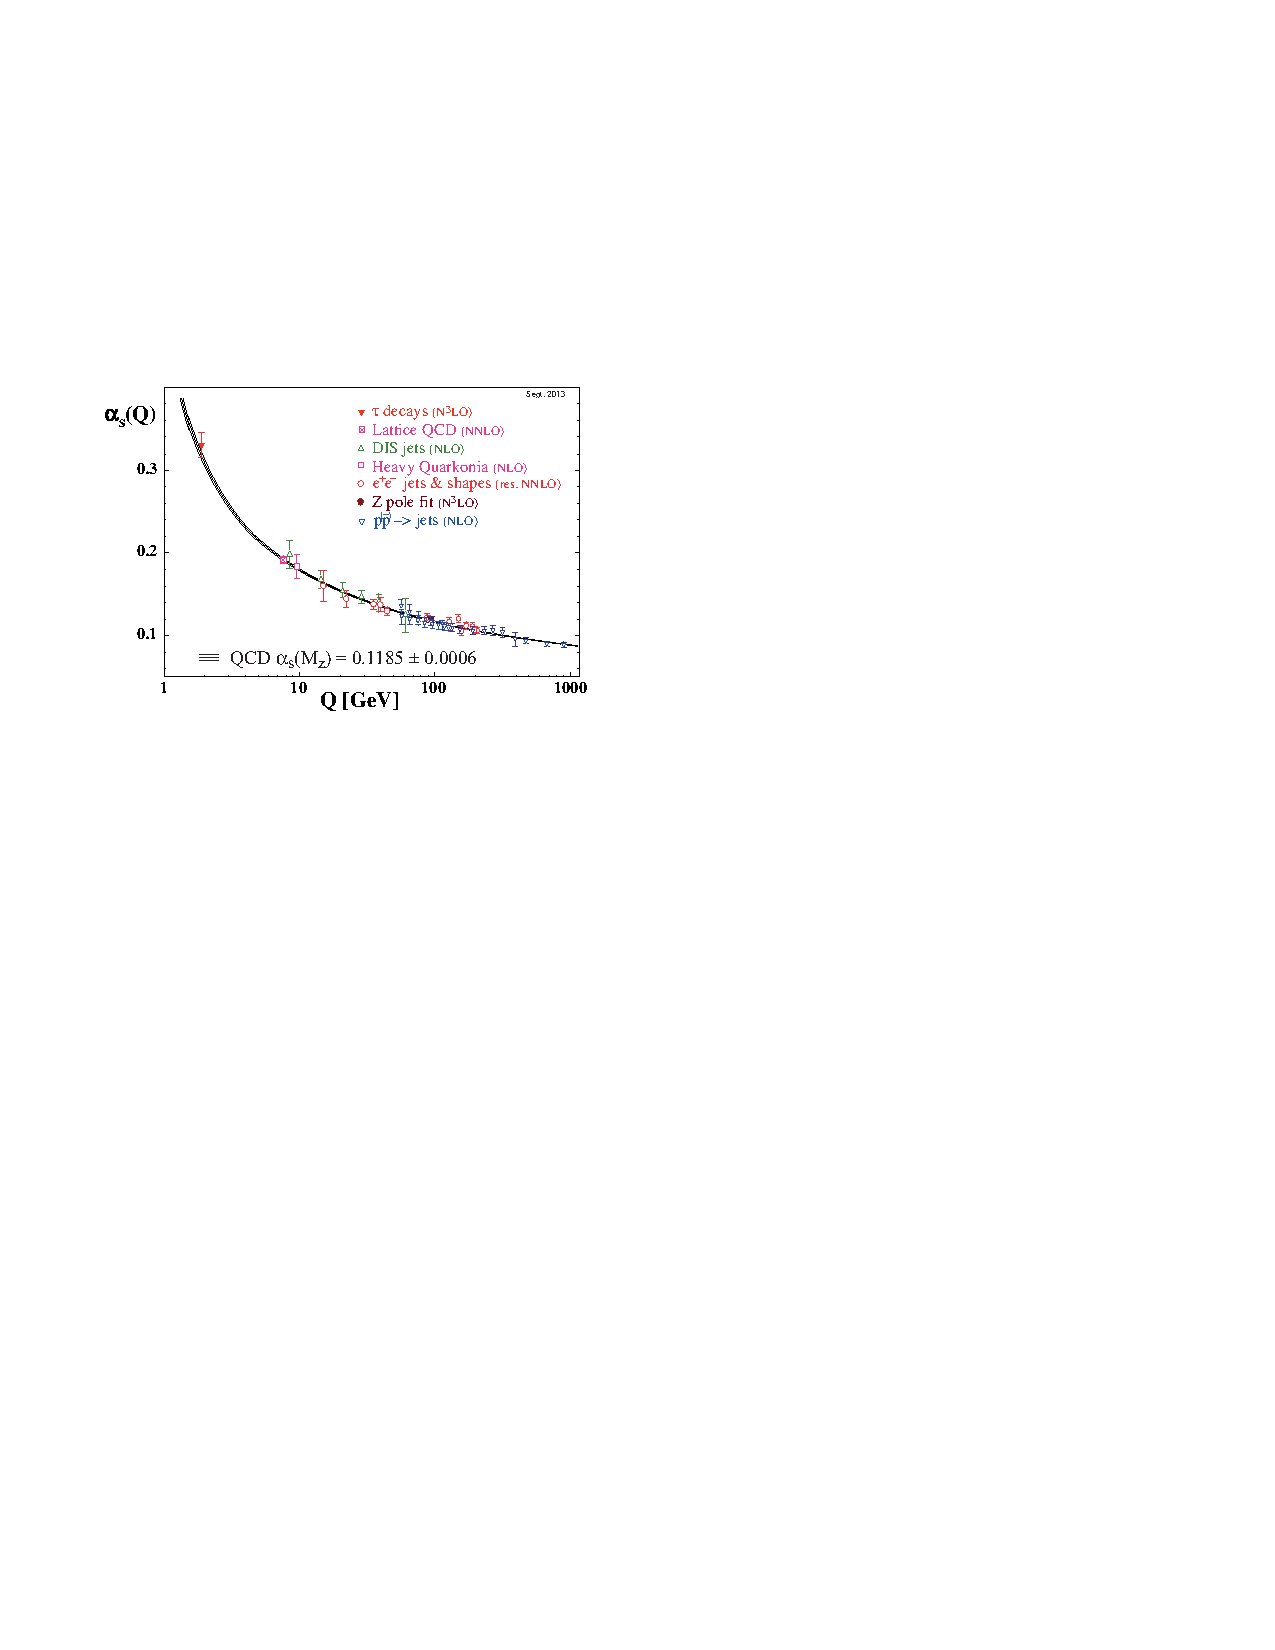
\includegraphics{Figures/alpha_s.pdf}
		%\rule{35em}{0.5pt}
	\caption[Strong force coupling constant]{Summary of measurement of strong coupling constant $\alpha_s$\citep{Agashe:2014kda} }
	\label{fig:alpha_s}
\end{figure}

	However, perturbative QCD cannot be used if the momentum transfer values are small and the coupling constant becomes large. This phenomenon is called confinement and it required different treatment for the quarks inside the proton. Internal structure of a proton is described using parton distribution functions which are determined through deep inelastic scattering experiments. Parton distribution functions for each of the partons inside a proton is shown in Figure \ref{fig:MSTW} made with one specific PDF function. Using DGLAP equations, it is possible to evolve the PDFs for any momentum transfer value which is described in detail in \citep{Campbell:2006wx} 

\begin{figure}[htbp]
	\centering
		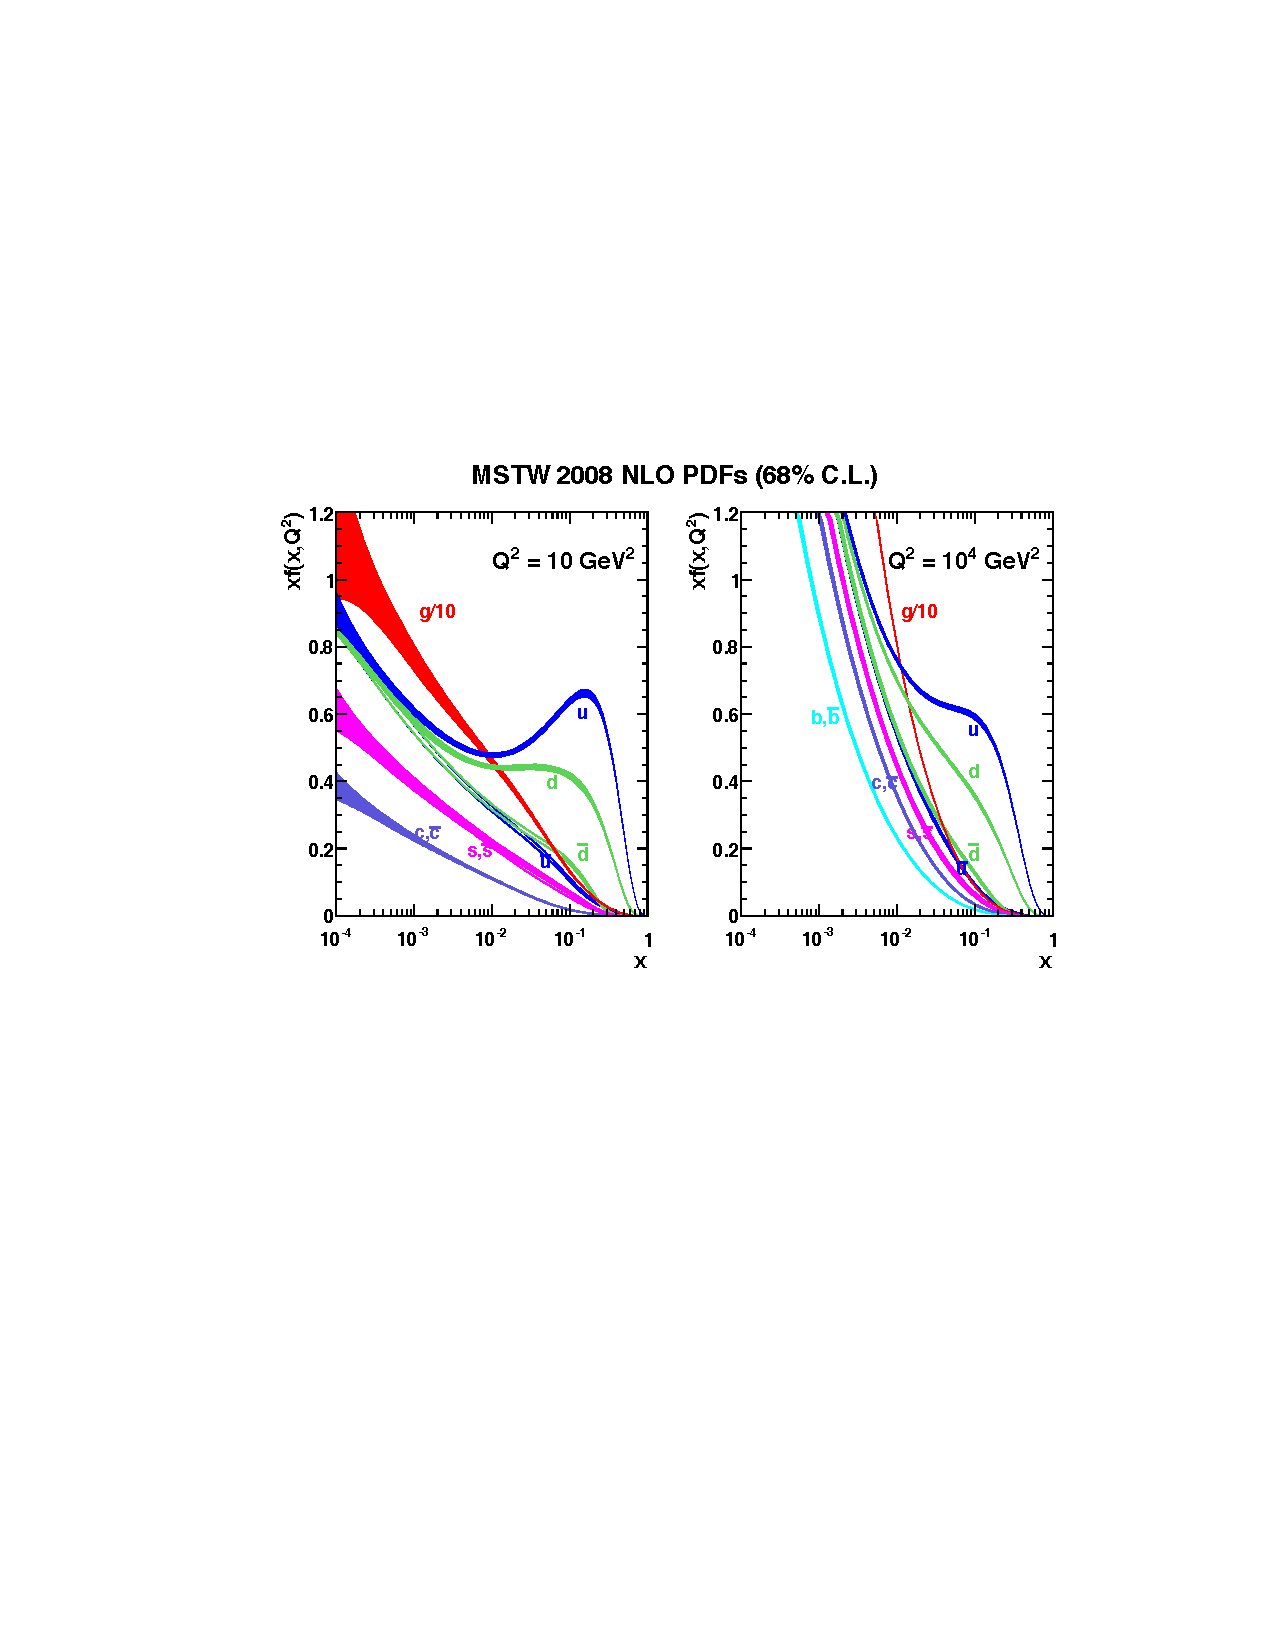
\includegraphics{Figures/MSTW.pdf}
		%\rule{35em}{0.5pt}
	\caption[Parton distribution functions for different momentum transfers]{Parton distribution functions calculated by the MSTW group for $Q=10$GeV and $Q=10^4$GeV \citep{Martin:2009iq}}
	\label{fig:MSTW}
\end{figure}


If we want to calculate the cross section for some process where there are two protons in the initial state and some interesting final state which we call X, according to \citep{Campbell:2006wx}, necessary steps are:
\begin{enumerate}
	\item Identify the leading order partonic processes that contribute to X
	\item Calculate the corresponding hard scattering cross section
	\item Determine the appropriate PDFs for initial state partons
	\item Make a specific choices for factorization($\mu_F$) and renormalization($\mu_R$) scales
	\item Perform integration over the fraction of momentum available for a given parton(x)  
\end{enumerate}



\begin{figure}[htbp]
	\centering
		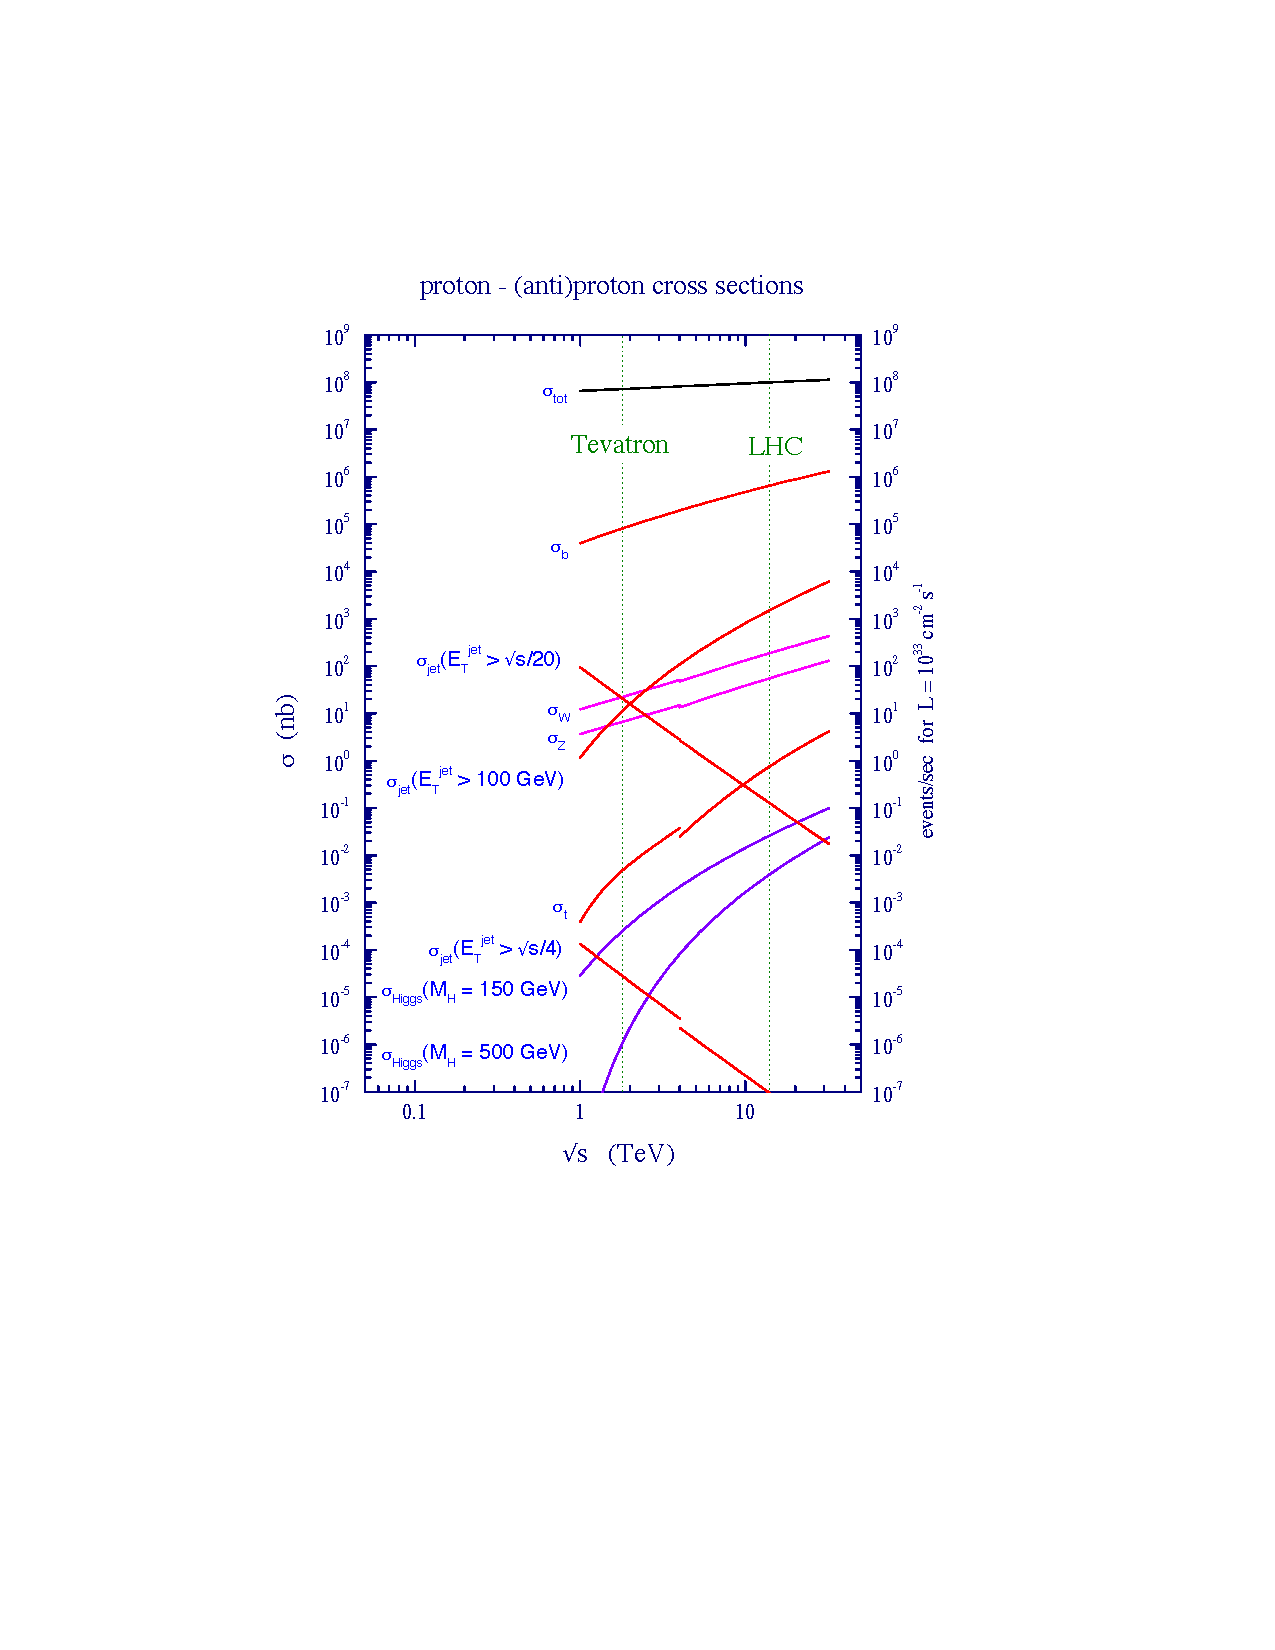
\includegraphics{Figures/pp_xsec.pdf}
		%\rule{35em}{0.5pt}
	\caption[Proton-proton cross sections]{Standard model cross sections as a function of center of mass energy.\citep{Campbell:2006wx} }
	\label{fig:pp_xsec}
\end{figure}

%-----------------------------------
%	SUBSECTION 2.2
%-----------------------------------

\subsection{Contributions to Wbb cross section}



%----------------------------------------------------------------------------------------
%	SECTION 3
%----------------------------------------------------------------------------------------

\section{Previous measurements}

	Previous measurements of W boson produced in association with b quarks have been performed on different experiments. However, the final states and phase space used in these measurements were different, which means that the results cannot be directly compared, but they can be compared with theoretical predictions. This process was measured for the first time at Tevatron with D0 and CDF experiments at $\sqrt{s} =$ 1.96 TeV. The CDF collaboration published its result in 2009 and the cross-section measured is that of “jets from b-quarks produced with a W boson”. The event selection is based on reconstructing a leptonically decaying W boson, and one or two jets where at least one has to be b-tagged. Events with jets from light quarks are vetoed with a cut on the secondary vertex mass. Contribution of other background events containing a b quark in final state (e.g. events with top quark) is estimated using Monte Carlo simulations. The measured cross section is 2.8 standard deviations higher than corresponding theoretical prediction. D0 collaboration published their result in 2012. with somewhat different phase space definition. The difference with respect to the CDF measurement consists in the inclusion of the events with 3 jets and reduced pseudorapidity range in which the measurement was performed. The measurement technique is similar to that of CDF, although b-tagging algorithms were slightly different. The measured cross section was in good agreement with the Standard model prediction.
	First measurements at the LHC were published by the ATLAS collaboration based on 36/pb of integrated luminosity at $\sqrt{s} =$ 7 TeV. One year later they improved their measurement using $4.6/$fb.\citep{Aad:2013vka} Selected events contain one reconstructed electron or muon, significant amount of missing transverse energy and one or two jets where exactly one is b-tagged. The phase space is divided in two regions, depending on the number of jets. Events with exactly 2 b jets and events with more than 2 jets are vetoed in order to suppress background events from top quark decay. The results are shown in Figure \ref{fig:atlas_tot}. The cross section measurement in the one jet region shows an excess corresponding to 1.5 standard deviations. In the two jet region, the measured cross section is in good agreement with theoretical predictions. A differential cross section measurement as a function of leading b jet transverse momentum has been performed for the first time and shown in figure \ref{fig:atlas_diff}. The cross section measurement in the one jet region is again higher that NLO predictions but within theoretical and experimental uncertainties. The cross section measured for the events with two jets is in good agreement with the theoretical prediction.
\begin{figure}[htbp]
	\centering
		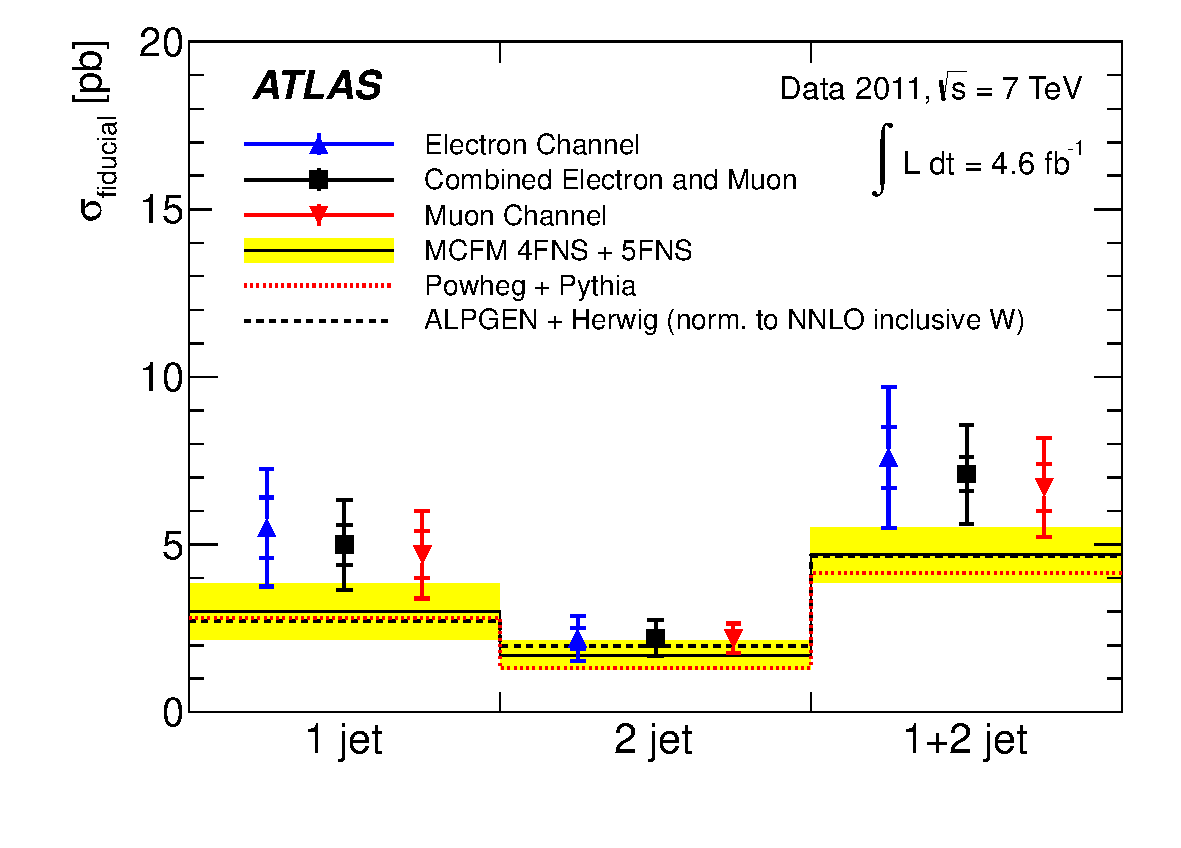
\includegraphics[width=0.7\linewidth]{Figures/atlas_total.pdf}
		%\rule{35em}{0.5pt}
	\caption[Atlas Wbb total cross section measurement]{Measured fiducial cross-sections in the electron, muon, and combined electron and muon channels. The cross-sections are given in the 1-jet, 2-jet, and 1+2-jet fiducial regions.\citep{Aad:2013vka} }
	\label{fig:atlas_tot}
\end{figure}

\begin{figure}
\centering
  \begin{subfigure}{.5\textwidth}
  	\centering
  	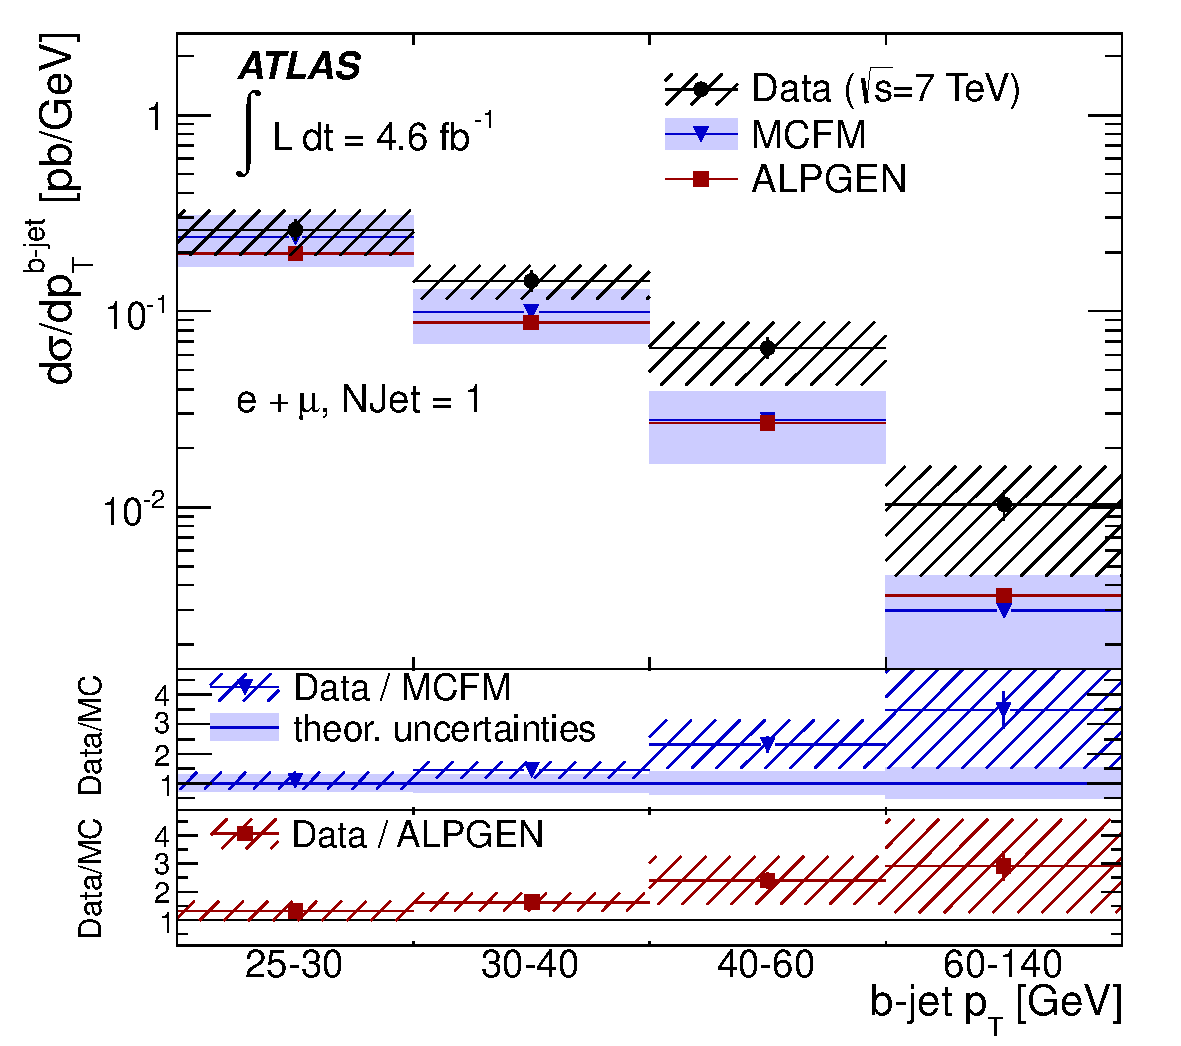
\includegraphics[width=\linewidth]{Figures/atlas_diff1j.pdf}
	\caption{}  
  	\label{fig:atlas_diff1j}
\end{subfigure}%
\begin{subfigure}{.5\textwidth}
  \centering
  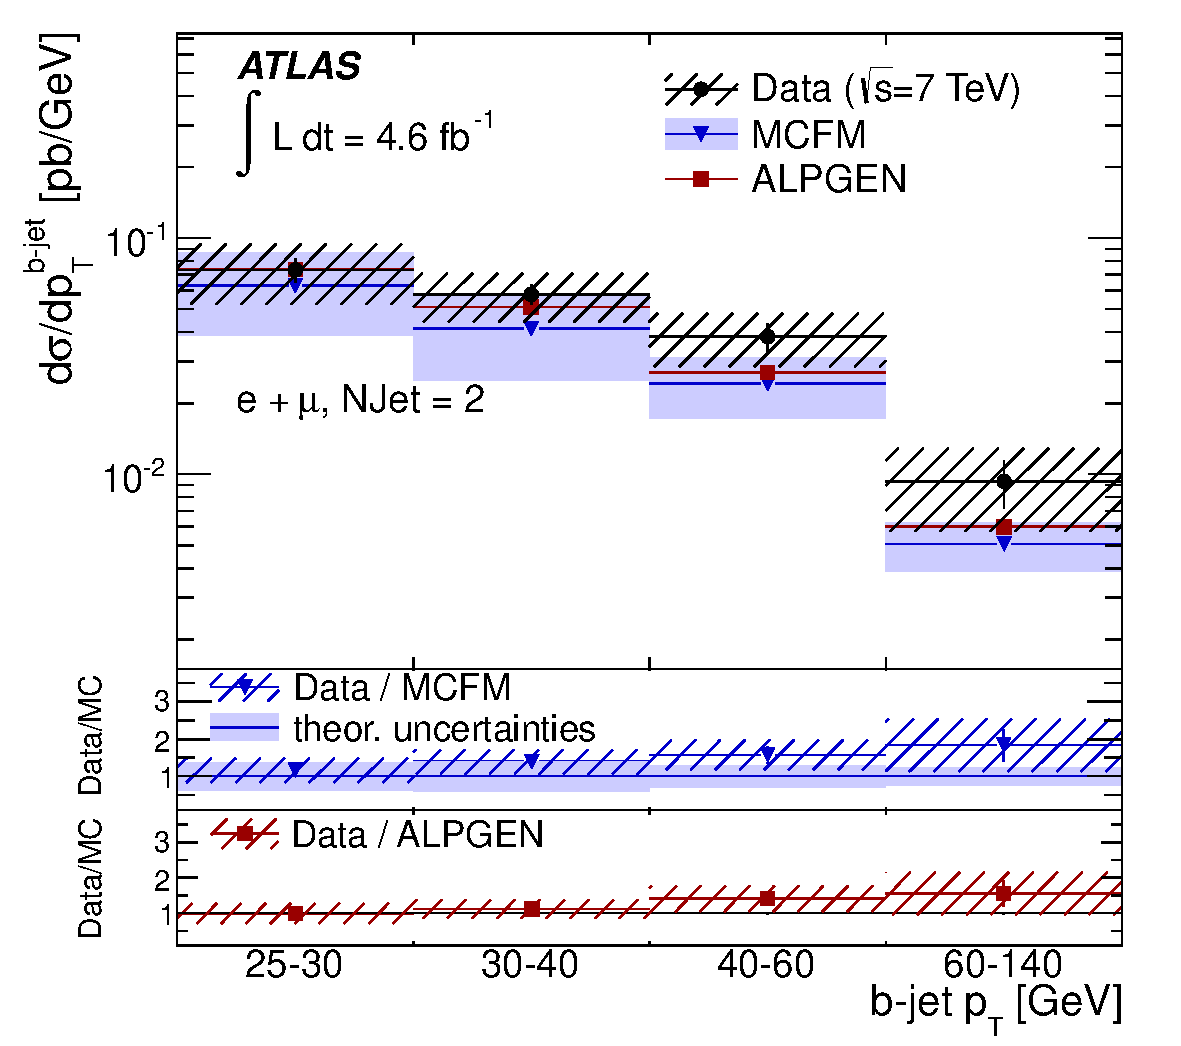
\includegraphics[width=\linewidth]{Figures/atlas_diff.pdf}
  \caption{}
  \label{fig:atlas_diff2j}
\end{subfigure}
\caption{Measured differential W+b-jets cross-sections as a function of leading b-jet $p_{T}$ in the 1-jet (\ref{fig:atlas_diff1j}) and 2-jet (\ref{fig:atlas_diff2j}) fiducial regions, obtained by combining the muon and electron channel results. \citep{Aad:2013vka}}
\label{fig:atlas_diff}
\end{figure}
	
	
The CMS collaboration published results corresponding to integrated luminosity of 5/fb. The measured events contained a muon and missing transverse energy in the final state, together with two b-tagged jets. The measured cross section is in excellent agreement with the Standard model prediction.\citep{Chatrchyan:2013uza}

\begin{figure}[htbp]
	\centering
		\includegraphics{Figures/cms_total.pdf}
		%\rule{35em}{0.5pt}
	\caption[CMS Wbb total cross section measurement]{Standard model cross sections as a function of center of mass energy.\citep{Aad:2013vka} }
	\label{fig:cms_total}
\end{figure}